\documentclass[]{scrartcl}

\usepackage{graphicx}
%%\usepackage{amsmath}

\usepackage{natbib}

%opening
\title{PHY 982 - HW 2}
\author{Xingze Mao \\ Zachary Matheson \\ Thomas Redpath}
\date{}

\begin{document}

\maketitle

\section*{Reaction and OMP parameters}

\begin{equation}
	^{100} \mathrm{Mo} (p,p) ^{100} \mathrm{Mo}
	\label{eq:therxn}
\end{equation}

\begin{equation}
	^{100} \mathrm{Mo} (n,n) ^{100} \mathrm{Mo}
	\label{eq:therxn}
\end{equation}


\begin{table}
\centering
	\begin{tabular}{ | c | c  c | }
\hline
	Projectile 1 & $p$ & $ J ^{\pi} = 1/2 ^+ $ \\
	Projectile 2 & $n$ & $ J ^{\pi} = 1/2 ^+ $ \\
\hline
	Target & $ ^{100} \mathrm{Mo} $ & $ J ^{\pi} = 0 ^+ $ \\
\hline
	\end{tabular}
	\caption{Entrance partition quantum numbers}
	\label{tab:entrance}
\end{table}

\section*{Proton elastic scattering: $E=5,50$ MeV}

\section*{Neutron elastic scattering: $E=5,50$ MeV}


%\begin{figure}
%\centering
%	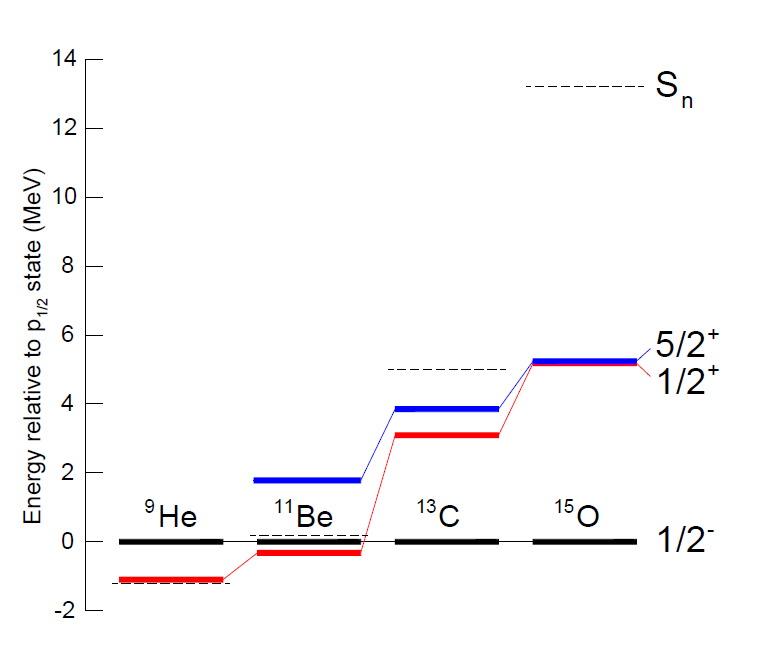
\includegraphics[width=\textwidth]{figures/n7isotones.png}
%	\caption{The evolution of single particl levels for the $N=7$ isotones (from \citep{Schmitt2011}). It is clear that the $1/2 ^+$ state drops below the $1/2 ^-$ in energy for $^{11}$Be.}
%	\label{fig:n7isotones}
%\end{figure}


%\begin{figure}
%\centering
%	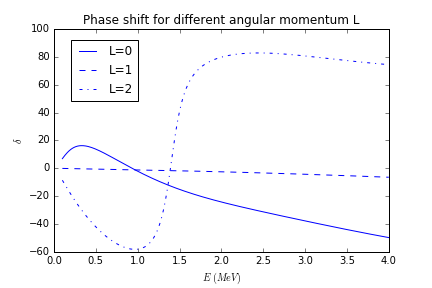
\includegraphics[width=0.85\textwidth]{figures/phase.png}
%	\caption{Phase shifts $\delta(E)$ for $l=0,1,2$. A weak resonance appears for $l=2$ near $E=1.4$ MeV with a width of $\sim 260$ keV.}
%	\label{fig:phase}
%\end{figure}

\clearpage


%%\bibliographystyle{apj}
%\bibliographystyle{plain}
%\bibliography{ref}

\end{document}
